\documentclass[border=0.125cm]{standalone}
\usepackage{tikz}
\usetikzlibrary{positioning}
\begin{document}

\definecolor{dense_node}{RGB}{196,225,144}
\definecolor{dropout_node}{RGB}{222,222,222}

\tikzset{%
  every neuron/.style={
    circle,
    draw,
    fill=dropout_node,
    opacity=0.3,
    minimum size=1cm
  },
  every line/.style={
    draw,
    opacity=0.3,
    minimum size=1cm
  },
  highlight neuron/.style={
    circle,
    draw,
    fill=dense_node,
    minimum size=1cm
  },
  highligh line/.style={
    draw,
    opacity=1,
    minimum size=1cm
  },
  neuron missing/.style={
    draw=none, 
    fill=none,
    scale=4,
    text height=0.333cm,
    execute at begin node=\color{black}$\vdots$
  },
}

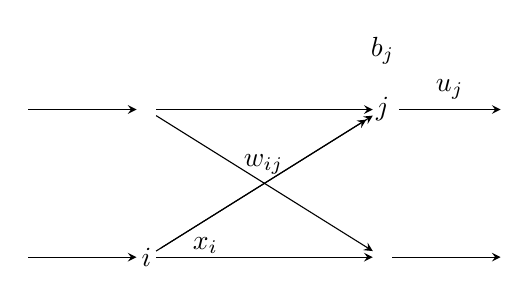
\begin{tikzpicture}[x=1.5cm, y=1.5cm, >=stealth]

\foreach \m/\l [count=\y] in {1,2}
  \node [every neuron/.try, neuron \m/.try] (input-\m) at (0,2.5-\y*1.25) {};

\foreach \m [count=\y] in {1, 2}
  \node [every neuron/.try, neuron \m/.try ] (hidden1-\m) at (2,2.5-\y*1.25) {};

% \foreach \m/\l [count=\y] in {missing,1,2,missing}
%   \node [every neuron/.try, neuron \m/.try] (input-\m) at (0,2.5-\y*1.25) {};

% \foreach \m [count=\y] in {missing, 1, 2, missing}
%   \node [every neuron/.try, neuron \m/.try ] (hidden1-\m) at (2,2.5-\y*1.25) {};
  
% \foreach \m [count=\y] in {missing, 1, 2, missing}
%   \node [every neuron/.try, neuron \m/.try ] (hidden2-\m) at (4,2.5-\y*1.25) {};

% \foreach \m [count=\y] in {1}
%   \node [every neuron/.try, neuron \m/.try ] (output-\m) at (6,-2) {};

\foreach \l [count=\i] in {1,2}
  \draw [<-, every line/.try] (input-\i) -- ++(-1,0)
    node [above, midway] {};

% \foreach \l [count=\i] in {1,n}
%   \node [above] at (hidden-\i.north) {$H_\l$};

% \foreach \l [count=\i] in {j,j+1}
%   \draw [->, every line/.try] (hidden1-\i) -- ++(1,0)
%     node [above, midway] {$u_{\l}$};

\foreach \i in {1,...,2}
  \foreach \j in {1,...,2}
    \draw [->, every line/.try] (input-\i) -- (hidden1-\j);
    
% \foreach \i in {1,...,2}
%   \foreach \j in {1,...,2}
%     \draw [->, every line/.try] (hidden1-\i) -- (hidden2-\j);

% \foreach \i in {1,...,4}
%   \foreach \j in {1}
%     \draw [->, every line/.try] (hidden2-\i) -- (output-\j);

% \foreach \l [count=\x from 0] in {Indata-, Tätt, Tätt, Utdata-}
%   \node [align=center, above] at (\x*2,2) {\l \\ lager};

% Mark certain nodes and corresponding lines
\node [highlight neuron/.try, neuron 1/.try ] (highlight-1) at (0,2.5-2*1.25) {$i$};
\node [highlight neuron/.try, neuron 2/.try ] (highlight-2) at (2,2.5-1*1.25) {$j$};
\node at (2,2.5-1*1.25+0.5) {$b_j$};
\draw [->, highlight line/.try] (highlight-1) -- (highlight-2)
    node [above, midway] {$w_{ij}$};
\node at (0+0.5,2.5-2*1.25+0.1) {$x_{i}$};
\draw [->, highlight line/.try] (highlight-2) -- ++(1,0)
    node [above, midway] {$u_{j}$};
\draw [->, every line/.try] (hidden1-2) -- ++(1,0) {};

\end{tikzpicture}

\end{document}